\section{Configurazione}\label{configurazione}

Questa sezione è dedicata alla persona delegata alla configurazione di \progetto.
Su richiesta di \II, tutti i servizi sono stati configurati sotto forma di \gloss{container}. È quindi possibile avviarli su macchine fisiche differenti, ma collegate in rete fra loro, con \gloss{Docker}.\\
Sempre sotto richiesta di \II\ viene utilizzato \gloss{Rancher} come software per la gestione dei container, quindi questa guida verterà principalmente sulla configurazione di \progetto\ utilizzando questa tecnologia.

\subsection{Requisiti di sistema}

	Non sono necessari particolari requisiti in modo da poter configurare e utilizzare il nostro prodotto, tuttavia valgono i requisiti minimi dei sistemi di terze parti che vengono utilizzati da \progetto.

	\subsubsection{Software}
		\begin{itemize}
			\item \textbf{Docker}\footnote{\url{https://docs.docker.com/v17.09/datacenter/ucp/2.1/guides/admin/install/system-requirements}}: è necessario avere installata e configurata correttamente almeno la versione v18.09.
			\item \textbf{Docker Compose}\footnote{\url{https://docs.docker.com/compose/install/}}:  nel caso si decidesse di utilizzare \gloss{Docker Compose} per l'avvio dei container è consigliata l'installazione e configurazione corretta della versione v3.7.
			\item \textbf{Kubernetes}\footnote{\url{https://kubernetes.io/docs/setup/independent/install-kubeadm}}: nel caso si decidesse di utilizzare \gloss{Kubernetes} per la gestione dei container è consigliata l'installazione e configurazione corretta della versione v1.13.
			\item \textbf{Rancher}\footnote{\url{https://rancher.com/docs/rancher/v2.x/en/installation/requirements/}}: nel caso si decidesse di utilizzare Rancher per la gestione grafica di oggetti Kubernetes contenenti i container Docker, è consigliata l'installazione e configurazione della versione v2.1.4.
			\item \textbf{Kafka}\footnote{\url{https://docs.confluent.io/current/installation/system-requirements.html}}: è necessario avere installata e configurata correttamente almeno la versione v2.12.
			\item \textbf{GitLab}\footnote{\url{https://git.ucd.ie/help/install/requirements.md}}: durante lo sviluppo di \progetto~abbiamo fatto riferimento alla versione v11.7.
			\item \textbf{Redmine}\footnote{%
			\url{https://www.easyredmine.com/faq/technical-info/176-hardware-and-software-requirements-for-server-solution}}: durante lo sviluppo di \progetto~abbiamo fatto riferimento alla versione v3.3.9.
		\end{itemize}

	GitLab e Redmine sono componenti esterne a \progetto, tuttavia vengono citate in quanto è possibile configurare tutto il progetto in un ambiente unico.\par
	Le versioni specificate possono essere trovate anche tra i requisiti di vincolo nel documento \AdRd.

	\subsubsection{Hardware}
	Per \progetto\ non sono necessari ulteriori requisiti a livello hardware particolari se non quelli di cui hanno bisogno i software precedentemente elencati.
	Unicamente per \progetto, senza tenere conto di servizi di terze parti, i requisiti sono:
	\begin{itemize}
		\item OS: Ubuntu 16.04 (o successive versioni)
		\item RAM: 3GB
		\item CPU: IntelCore i3 con 2.1 GHz (o processori con potenza analoga o superiore)
		\item Spazio su disco: 2GB
		\item Completa possibilità di comunicazione in rete dei container
	\end{itemize}

\subsection{Mappatura delle porte}
Per la configurazione di ciascun tipo servizio abbiamo deciso di dare un range di porte da poter esporre in modo tale da effettuare una separazione logica.\\
Questa regola non influisce col corretto funzionamento di \progetto, ma è solamente per non assegnare le porte in modalità casuale e facilitare le analisi di eventuali errori, la manutenzione e l'aggiunta futura di nuovi servizi.
La suddivisione delle porte è la seguente:
%TODO verificare bene questo e che sia implementato in questa maniera
\begin{table}[H]
	\centering
	\begin{paddedtablex}[1.3]{\textwidth}{YYY}
		\thead{Servizio} & \thead{Porta inizio} & \thead{Porta fine}\\\toprule
		Software di terze parti& 30000& 30029\\
		Kafka e servizi correlati& 30030& 30059\\
		Producer& 30060& 30089\\
		Consumer& 30090& 30119\\
		Gestore Personale& 30120& 30149\\\bottomrule
	\end{paddedtablex}
	\caption{Suddivisione del range delle porte a disposizione su Rancher}
\end{table}

La suddivisione che abbiamo utilizzato, durante lo sviluppo e la consegna del progetto, prevede la seguente esposizione delle porte:

%TODO verificare bene questo e che sia implementato in questa maniera
\begin{table}[H]
	\centering
	\begin{paddedtablex}[1.3]{\textwidth}{YYY}
		\thead{Servizio} & \thead{Porta interna} & \thead{Porta esposta}\\\toprule
		Redmine& 3000& 30000\\
		GitLab& 80& 30001\\
		Kafka& 9092& 30030\\
		Producer GitLab& 5000& 30060\\
		Producer Redmine& 5000& 30061\\
		Consumer Telegram& 80& 30090\\
		Consumer Email& 80& 30091\\
		Producer Gestore Personale& 5000& 30120\\
		Consumer Gestore Personale& 80& 30121\\\bottomrule
	\end{paddedtablex}
	\caption{Configurazione delle porte in fase di sviluppo e consegna}
	\label{TabellaPorteEsposte}
\end{table}

Le specifiche relative alla configurazione delle porte in Rancher possono essere trovate nella documentazione presente sul sito di Rancher nella pagina dedicata\footnote{\url{https://rancher.com/docs/rancher/v2.x/en/installation/references/}}.

\subsection{Suddivisione dei container ed immagini utilizzate}
Come detto in precedenza, su consiglio di \II, \progetto\ è stato sviluppato con l'utilizzo di Rancher per la gestione dei container.\\
I container sono stati suddivisi in modo tale da utilizzare un unico \gloss{Cluster} (nel nostro caso chiamato Butterfly), vari \gloss{Namespace} per separare i servizi fra loro e i \gloss{Pod}, che rappresentano ciascuno un container.
Le immagini utilizzate sono tutte presenti in DockerHub, incluse quelle dei \gloss{Producer} e dei \gloss{Consumer} che sono state create utilizzando build automatiche innescate ad ogni \gloss{push} nella repository del codice.
\newpage
La configurazione che abbiamo utilizzato all'interno del Cluster \progetto\ è:
\begin{itemize}
	\item Namespace: \texttt{gitlab}
	\begin{itemize}
		\item Pod: \texttt{gitlab} (immagine: \texttt{gitlab/gitlab-ce:latest}\footnote{\url{https://hub.docker.com/r/gitlab/gitlab-ce/}})%\footnote{Non sono necessari ulteriori servizi per GitLab in quanto l'immagine ufficiale contiene tutte le componenti necessarie per il suo corretto funzionamento.}
	\end{itemize}

	\item Namespace: \texttt{redmine}
	\begin{itemize}
		\item Pod: \texttt{redmine} (immagine: \texttt{redmine:3.3.9}\footnote{\url{https://hub.docker.com/_/redmine}})
		\item Pod: \texttt{postgres-redmine} (immagine: \texttt{postgres:11-alpine}\footnote{\url{https://hub.docker.com/_/postgres}})
	\end{itemize}

	\item Namespace: \texttt{producer}
	\begin{itemize}
		\item Pod: \texttt{producer-gitlab} (immagine: \texttt{alphasix/producer-gitlab:master}\footnote{\url{https://hub.docker.com/r/alphasix/producer-gitlab}})
		\item Pod: \texttt{producer-redmine} (immagine: \texttt{alphasix/producer-redmine:master}\footnote{\url{https://hub.docker.com/r/alphasix/producer-redmine}})
	\end{itemize}

	%TODO Successivamente aggiungere pod di monitoraggio
	\item Namespace: \texttt{kafka}
	\begin{itemize}
		\item Pod: \texttt{kafka-kafka} (immagine: \texttt{confluentinc/cp-kafka:4.0.1-1}\footnote{\url{https://hub.docker.com/r/confluentinc/cp-kafka/}})
		\item Pod: \texttt{kafka-zookeeper} (immagine: \texttt{confluentinc/cp-zookeeper:4.1.1}\footnote{\url{https://hub.docker.com/r/confluentinc/cp-zookeeper/}})
	\end{itemize}

	%TODO successivamente da vedere se è in un unico pod oppure se in pod separati
	\item Namespace: \texttt{gestore-Personale}
	\begin{itemize}
		\item Pod: \texttt{gestore-personale} (immagine: \texttt{alphasix/gestore-personale:master}\footnote{\url{https://hub.docker.com/r/alphasix/gestore-personale}})
		\item Pod: \texttt{mongo} (immagine: \texttt{bitnami/mongodb:latest}\footnote{\url{https://hub.docker.com/r/bitnami/mongodb/}})
	\end{itemize}

	\item Namespace: \texttt{consumer}
	\begin{itemize}
		\item Pod: \texttt{consumer-telegram} (immagine: \texttt{alphasix/consumer-telegram:master}\footnote{\url{https://hub.docker.com/r/alphasix/consumer-telegram}})
		\item Pod: \texttt{consumer-email} (immagine: \texttt{alphasix/consumer-email:master}\footnote{\url{https://hub.docker.com/r/alphasix/consumer-email}})
	\end{itemize}
\end{itemize}

%TODO lo facciamo? magari per la seconda relase
% All'interno della repository è possibile trovare un file in formato .yml conforme agli standard del docker compose per poter istanziare l'ambiente. Inoltre sono presenti i Dockerfile che permettono di effettuare la build di ciascuno dei componenti che abbiamo sviluppato.

\subsection{Configurazione webhook}
Per il corretto invio dei \gloss{webhook} (in formato \gloss{JSON}) da parte dei software che comunicano con i nostri Producer, è necessaria una breve configurazione delle applicazioni che dialogano con i Producer (GitLab e Redmine) spiegata nel dettaglio nei prossimi paragrafi.

	\subsubsection{Redmine}
	\paragraph{Configurazione del plugin}
	Per poter inviare un webhook con Redmine è necessario installare un \gloss{plugin} esterno chiamato \texttt{redmine\_webhook}\footnote{\url{https://github.com/suer/redmine_webhook.git}}.
	Per installarlo è necessario scaricarlo (tramite il comando \texttt{git clone} ad esempio) nella cartella \texttt{/plugins/redmine}.
	Non sono necessarie ulteriori configurazioni in quanto questo software è di tipo \gloss{plug and play}.
	Per verificare la corretta integrazione con Redmine, controllare da un profilo con privilegi amministratore che nella sezione \texttt{Settings > Plugins} sia presente il plugin appena scaricato.
	\begin{figure}[H]
		\centering
		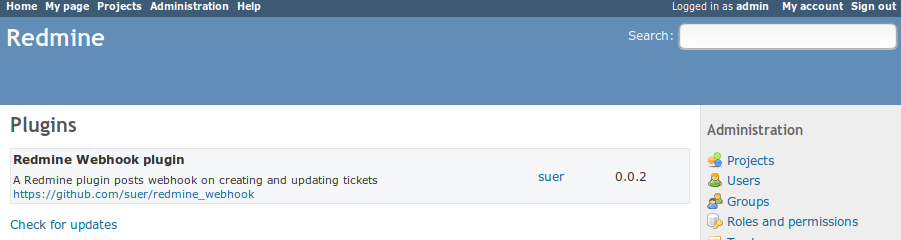
\includegraphics[width=14cm]{img/redmine_webhook_admin.png}
		\caption{Lista plugin configurati}
	\end{figure}

	%Questo plugin implementa il concetto di Hook offerto dalla API di Redmine, inviando a un determinato URL un \gloss{payload} costituito da un file JSON quando un evento si innesca, contenente le informazioni relative a tale evento.	Queste istruzioni saranno contenute anche nel README della repository sul quale è stato versionato il codice.

	\paragraph{Configurazione destinazione}
	Per aggiungere una destinazione del webhook per un progetto, andare nella sezione relativa a quest'ultimo all'interno del menu del progetto selezionato (\texttt{Settings > Webhook}).\\
	Nell'area di input aggiungere l'indirizzo di destinazione e premere ``Add''. Nel caso si volesse rimuovere un indirizzo precedentemente inserito allora premere ``Remove''.
	\begin{figure}[H]
		\centering
		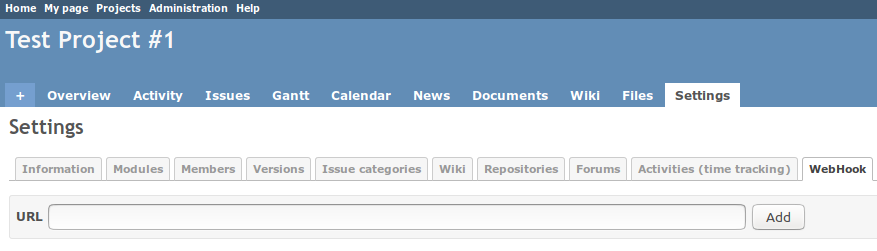
\includegraphics[width=14cm]{img/redmine_webhook_menu.png}
		\caption{Menu plugin \texttt{redmine\_webhook}}
	\end{figure}
	\paragraph{Eventi supportati}
	Per Redmine gli eventi supportati sono:
	\begin{itemize}
		\item Issue\footnote{Il plugin \texttt{redmine\_webhook} offre l'invio dei webhook solamente da parte degli eventi relativi alle Issue}
	\end{itemize}

	\subsubsection{GitLab}
	\paragraph{Configurazione webhook nella rete locale}
	È necessario abilitare l'invio dei webhook a dispositivi presenti nella stessa rete dalla parte amministrativa.
	Questo può essere effettuato accedendo con un account con privilegi amministratore all'indirizzo:
	\begin{center}
		\texttt{\url{/admin/application_settings/network}}
	\end{center}
	Per abilitare questa funzionalità, è necessario cliccare sul riquadro visibile nell'immagine \ref{ConfigWebGit} e che si trova all'indirizzo sopra indicato.
	\begin{figure}[H]
		\centering
		
\includegraphics[width=13cm]{img/webhook_gitlab_setup.png}\\
		\caption{Configurazione webhook con destinazione in rete locale}
		\label{ConfigWebGit}
	\end{figure}
	Ulteriori informazioni a riguardo possono essere trovate nella pagina\footnote{\url{https://docs.gitlab.com/ee/security/webhooks.html}} relativa a tale argomento nella sezione relativa alla documentazione di GitLab.

	\paragraph{Configurazione destinazione}
	Successivamente si può aggiungere un indirizzo di destinazione di un webhook al progetto in \texttt{Settings > Integrations}.
	Da qui si possono selezionare gli eventi di interesse per i quali i webhook verranno attivati.\\
	%NB: c'è scritto sotto quali sono quelli supportati
	%(attenzione: \progetto~non supporta qualunque tipo di evento, ma solamente quelli richiesti da \II).\\
	Nel campo relativo all'URL di destinazione inserire l'indirizzo con la relativa porta (nel nostro caso quella specificata nella Tabella \ref{TabellaPorteEsposte}) su cui il Producer GitLab è in ascolto.
	\paragraph{Eventi supportati}
	Per GitLab gli eventi supportati sono:
	\begin{itemize}
		\item Push events
		\item Comments
		\item Issues events
	\end{itemize}

\subsection{Configurazione servizi \progetto}\label{var}

	\subsubsection{Producer}
	Per i Producer è possibile impostare nell'apposito file di configurazione le variabili relative.

	Per il Producer di Redmine i campi sono:
	\begin{itemize}
		\item\texttt{"kafka":\{"bootstrap\_servers"\}}: indirizzo e porta dell'istanza di Kafka disponibile.
		% \item\texttt{BUTTERFLY\_PRODUCER\_KAFKA\_BOOTSTRAP\_SERVERS}: indirizzo e porta dell'istanza di Kafka disponibile.
		\item\texttt{"redmine":\{"ip"\}}: indirizzo dell'istanza di Redmine disponibile.
		% \item\texttt{BUTTERFLY\_PRODUCER\_REDMINE\_IP}: indirizzo dell'istanza di Redmine disponibile.
		\item\texttt{"redmine":\{"port"\}}: porta dell'istanza di Redmine disponibile.
		% \item\texttt{BUTTERFLY\_PRODUCER\_REDMINE\_PORT}: porta dell'istanza di Redmine disponibile.
	\end{itemize}

	Per il Producer di GitLab i campi sono:
	\begin{itemize}
		\item\texttt{"kafka":\{"bootstrap\_servers"\}}: indirizzo e porta dell'istanza di Kafka disponibile.
		% \item\texttt{BUTTERFLY\_PRODUCER\_KAFKA\_BOOTSTRAP\_SERVERS}: indirizzo e porta dell'istanza di Kafka disponibile.
		\item\texttt{"gitlab":\{"ip"\}}: indirizzo dell'istanza di GitLab disponibile.
		% \item\texttt{BUTTERFLY\_PRODUCER\_GITLAB\_IP}: indirizzo dell'istanza di GitLab disponibile.
		\item\texttt{"gitlab":\{"port"\}}: porta dell'istanza di GitLab disponibile.
		% \item\texttt{BUTTERFLY\_PRODUCER\_GITLAB\_PORT}: porta dell'istanza di GitLab disponibile.
	\end{itemize}

	\subsubsection{Consumer}\label{var_consumer}
	Per i Consumer, come per i Producer, è possibile impostare le variabili tramite un file di configurazione.
	Queste sono, per il Consumer di Telegram:
	\begin{itemize}
		\item\texttt{"kafka":\{"bootstrap\_servers"\}}: indirizzo e porta dell'istanza di Kafka disponibile.
		% \item\texttt{BUTTERFLY\_CONSUMER\_KAFKA\_BOOTSTRAP\_SERVERS}: indirizzo e porta dell'istanza di Kafka disponibile.
		\item\texttt{"telegram":\{"token\_bot"\}}: \gloss{ID} del Bot di Telegram che inoltra la notifica.
		% \item\texttt{BUTTERFLY\_CONSUMER\_TELEGRAM\_BOT}: \gloss{ID} del Bot di Telegram che inoltra la notifica.
	\end{itemize}

	Per il Consumer Email, invece:
	\begin{itemize}
		\item\texttt{"kafka":\{"bootstrap\_servers"\}}: indirizzo e porta dell'istanza di Kafka disponibile.
		% \item\texttt{BUTTERFLY\_CONSUMER\_KAFKA\_BOOTSTRAP\_SERVERS}: indirizzo e porta dell'istanza di Kafka disponibile.
		\item\texttt{"email":\{"sender"\}}: indirizzo email che inoltra l'email.
		% \item\texttt{BUTTERFLY\_CONSUMER\_EMAIL\_SENDER}: email che inoltra la notifica.
		\item\texttt{"email":\{"psw"\}}: password della casella email.
		% \item\texttt{BUTTERFLY\_CONSUMER\_EMAIL\_PSW}: password della casella email.
	\end{itemize}

	È inoltre possibile impostare la password dell'indirizzo email tramite la variabile:
	\begin{itemize}
		\item\texttt{BUTTERFLY\_CONSUMER\_EMAIL\_PSW}: password della casella email.
	\end{itemize}

	\subsubsection{Gestore Personale}
	Per il Gestore Personale, come per i Producer e per i Consumer, è possibile impostare le variabili di file di configurazione. \par

	Per la componente Producer del Gestore Personale queste sono:
	\begin{itemize}
		\item\texttt{"kafka":\{"bootstrap\_servers"\}}: indirizzo e porta dell'istanza di Kafka disponibile.
		% \item\texttt{BUTTERFLY\_GP\_PRODUCER\_KAFKA\_BOOTSTRAP\_SERVERS}: indirizzo e porta dell'istanza di Kafka disponibile.
	\end{itemize}

	Per la componente Consumer del Gestore Personale queste sono:
	\begin{itemize}
		\item\texttt{"kafka":\{"bootstrap\_servers"\}}: indirizzo e porta dell'istanza di Kafka disponibile.
		% \item\texttt{BUTTERFLY\_GP\_CONSUMER\_KAFKA\_BOOTSTRAP\_SERVERS}: indirizzo e porta dell'istanza di Kafka disponibile.
	\end{itemize}


	\subsubsection{Kafka}
	Per l'utilizzo richiestoci da parte dell'azienda di Kafka non sono state necessarie ulteriori configurazioni oltre a quelle di default successive all'installazione.
